\chapter{Logistična regresija}

Se bo osnovnošolec Vinko uvrstil v drugi krog tekmovanja iz kemije? Se bo po srednji šoli vpisal na Kemijsko fakulteto? Ga bo zaposlilo podjetje, ki se ukvarja z biofarmacijo? Bo njegov košarkaški klub Olimpija premagal Crveno zvezdo to soboto? Se bo poročil s sosedovo Niko? Bo njegova ideja o tekočini, ki vsakih 35 minut spremeni barvo, uspela na Kickstarterju?

Morda smo s kakšnim od zgornjih vprašanj zašli, a na vsaj eno od naštetih vemo, da je nanj možno dovolj dobro odgovoriti. So pa to vprašanja, ki niso regresijska, oziroma je napoved kategoričnega tipa ``bo'' ali ``ne bo''. Še bolj natančno: za vsako od zgornjih vprašanj bi pravzaprav radi ocenili verjetnost, ali se bo nek dogodek zgodil. Recimo, zanima nas, s kakšno verjetnostjo se bo Vino poročil z Niko. In pa, s kakšno verjetnostjo bo njegov kicksterski projekt uspel.

Seveda bomo tudi tokrat napovedne modele, sedaj klasifikacijske, gradili iz podatkov. Za silo bi take podatke in s tem problem spremenili v regresijskega tako, da bi odgovore označili z vrednostjo 0 (dogodek se ni zgodil) ali 1 (dogodek se je zgodil), potem pa to vrednost obravnavali kot zvezno vrednost odvisne spremenljivke oziroma razreda $y$. Primer take obravnave nam kaže tabela~\ref{f:temperatura} s podatki o obiskovalcih ordinacije, ki jim je zdravnik izmeril telesno temperaturo in potem (seveda na podlagi dodatnih preiskav, ki pa jih tu ne podajamo) določil zdravstveno stanje. Naš cilj je zgraditi model, ki zdravstveno stanje oceni (samo) na podlagi telesne temperature.

\begin{table}[htbp]
\caption{Telesna temperatura in stanje pregledovanca, ki smo ga zapisali v numerični obliki kot razred $y$.}
\label{f:temperatura}
\begin{center}
\begin{tabular}{ccc}
\toprule
temperatura & stanje & $y$ \\
\midrule
36,5 & zdrav & 0 \\
36,6 & zdrav & 0 \\
36,8 & zdrav & 0 \\
36,9 & bolan & 1 \\
37,0 & zdrav & 0 \\
37,2 & bolan & 1 \\
37,5 & bolan & 1 \\
37,6 & bolan & 1 \\
39,5 & bolan & 1 \\
\bottomrule
\end{tabular}
\end{center}
\end{table}

Podatke predstavimo grafično (slika~\ref{f:class-linreg}) in si potem nanje drznemo vpeti linearno funkcijo $y=h(x)$. Najprej opazimo, da je zaloga vrednosti funkcije $h(x)$ neprimerna, saj gre ta od $-\infty$ do $\infty$. Na intervalu telesnih temperatur okoli točke $37^{\circ}$ ima funkcija sicer vrednost med 0 in 1. Pojavi pa se vprašanje, kako vrednost te linearne funkcije sploh interpretirati, oziroma kako jo pretvoriti v verjetnost. Spomnimo se, da vsaka verjetnostna funkcija vrača vrednosti med 0 in 1, naša linearna funkcija pa je omejena na ta interval samo v določenem območju vrednosti vhodnega atributa. Dodaten problem je še z osamelci, oziroma obiskovalci s skrajnimi vrednostnimi atributov. Če bi podatkom dodali še en primer bolnika z zelo visoko temperaturo, bi se naša funkcija precej spremenila in pomaknila v desno. Potrebujemo nek predpis, ki bi vrednosti take funkcije pretvoril v verjetnosti in jih morda blizu $y=0$ in $y=1$ malce zmehčal.

\begin{figure}[htbp]
\begin{center}
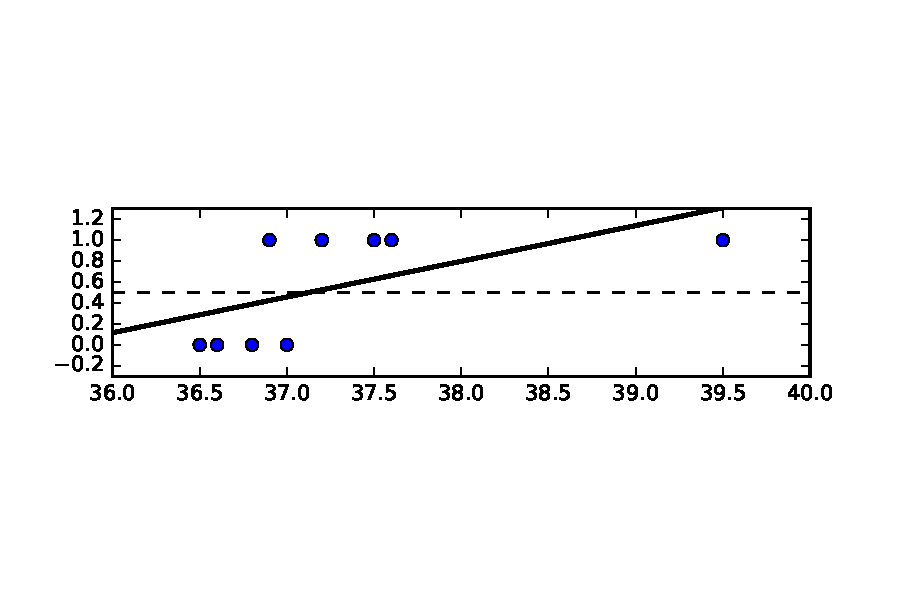
\includegraphics[width=10cm]{slike/class-linreg.pdf}
\caption{Poskus klasifikacije z linearno regresijo.}
\label{f:class-linreg}
\end{center}
\end{figure}

\section{Logistična funkcija}

Funkcija, ki jo bomo uporabili in ki neko realno število pretvori v število na intervalu [-1, 1], je logistična funkcija (slika~\ref{f:logistic-function}):
\begin{equation}
  g(z) = {1\over 1+e^{-z}}
\end{equation}

\begin{figure}[htbp]
\begin{center}
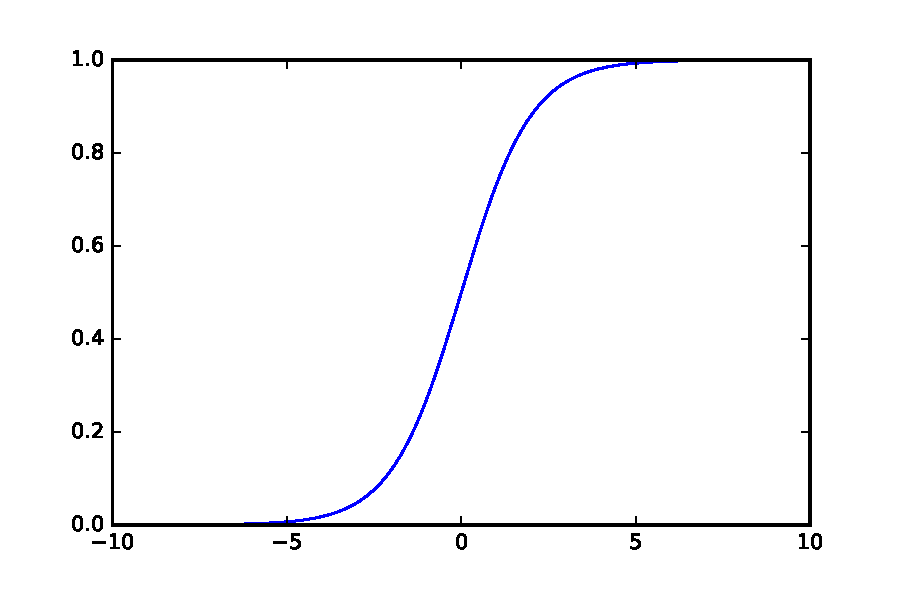
\includegraphics[width=10cm]{slike/logistic.pdf}
\caption{Logistična funkcija.}
\label{f:logistic-function}
\end{center}
\end{figure}

Logistična funkcija je zvezna, monotona, z $z\to -\infty$ konvergira proti 0 in z $z\to\infty$ proti 1. Je odvedljiva pri vseh vrednosti njenega parametra. Njen odvod je:
\begin{eqnarray}
  \frac{dg(z)}{dz} & = & \frac{d}{dz} \frac{1}{1+e^{-z}} \nonumber \\
  & = & \frac{1}{(1+e^{-z})^2} e^{-z} \nonumber \\
  & = & \frac{1}{1+e^{-z}}\frac{e^{-z}}{1+e^{-z}} \nonumber \\
  & = & \frac{1}{1+e^{-z}}\frac{1+e^{-z}-1}{1+e^{-z}} \nonumber \\
  & = & \frac{1}{1+e^{-z}}\big(1-\frac{1}{1+e^{-z}}\big) \nonumber \\
  & = & g(z)[1-g(z)]
\end{eqnarray}

\section{Logistična regresija}

Zapišimo sedaj naš klasifikacijski model. V osnovi bo to linearni model, torej utežena vsota vrednosti atributov. A tokrat jo bomo transformirali z logistično funkcijo, da bo vrednost modela izražala pripadnost (verjetnost) ciljnemu razredu:
\begin{eqnarray}
  h_\theta(x) & = & g(\theta_0+\theta_1 x_1+\theta_2 x_2+\ldots\theta_n x_n)
  \nonumber \\
  & = & g(\theta^T x) \nonumber \\
  & = & \frac{1}{1+e^{-\theta^T x}}
  \label{eq:logreg}
\end{eqnarray}

Model zaradi uporabe logistične funkcije imenujemo {\em logistična regresija}.

\section{Računanje verjetnosti razreda}

V nadaljevanju bomo torej logistično funkcijo uporabili tako, da nam bo naš model $h_{\theta}(x)$, ki je v osnovi linearni model, vračal vrednosti med 0 in 1. Še naprej bomo predpostavljali, da je naša razredna spremenljivka dvovrednostna, a privzeli, da je njena ciljna vrednost razred z oznako $y=1$ in da zanj model $h_{\theta}(x)$ vrača verjetnost tega razreda. K oznaki modela smo namenoma pripisali oznako za vektor parametrov $\theta$ in na ta način poudarili, da ti parametri tudi polno opredelijo naš model. Zapišemo torej lahko:
\begin{eqnarray}
  P(y=1|x;\theta) & = & h_\theta(x) \\
  P(y=0|x;\theta) & = & 1-h_\theta(x)
\end{eqnarray}
Izraz za $P(y=1|x;\theta)$ nam torej podaja verjetnost, da je razred primera, ki je opisan z vektorjem atributnih vrednosti $x$, enak 1. Oziroma podaja verjetnost, da neodvisna spremenljivka zavzame vrednost 1 pri opisu primera $x$ in parametrizaciji modela s parametri $\theta$. En sam izraz, ki združi zgornji enačbi v eno in ki podaja verjetnostno porazdelitev za spremenljivko $y$ je:
\begin{equation}
  p(y|x;\theta) = (h_\theta(x))^y(1-h_\theta(x))^{1-y}
\label{eq:log-prob}
\end{equation}
Pravilnost zgornjega izraza preveri tako, da za vrednost spremenljivke $y$ vstaviš enkrat $y=1$ in drugič $y=0$.

\section{Verjetje}

Izraz za $p(y|x;\theta)$ v enačbi~\ref{eq:log-prob} torej podaja verjetnost za določeno vrednost neodvisne spremenljivke in določen vektor atributnih vrednosti pri modelu, ki je podan z $\theta$. Sedaj pa si predstavljamo, da vrednosti elementov vektorja $\theta$ spreminjamo. Prav gotovo se bo na ta način tudi spreminjala verjetnost za dani razred pri izbranem primeru; enkrat bo ta verjetnost višja, drugič nižja.

Zamrznimo sedaj parametre modela $\theta$ in izračunajmo verjetnosti $L(\theta)$ pravih razredov $\vec{y}$ za primere v učni množici, ki jo opišemo z matriko atributnih vrednosti $X$. Predpostavljamo, da so primeri iz učne množice neodvisni in zato verjetnost za vrednosti spremenljivke $y$ za celotno učno množico lahko zapišemo kot produkt verjetnosti za vrednost $y$ za posamezne primere:
\begin{eqnarray}
  L(\theta) & = & p(\vec{y}|X;\theta) \nonumber\\
  & = & \prod_{i=1}^m p(y^{(i)}|x^{(i)};\theta) \nonumber\\
  & = & \prod_{i=1}^m h_\theta(x^{(i)})^{y^{(i)}}(1-h_\theta(x^{(i)}))^{1-y^{(i)}}
\end{eqnarray}

Kot smo označili v zgornji funkciji $L$, je ta verjetnost odvisna od parametrov modela $\theta$. Kakšen model bi želeli imeti? Tak, pri katerem je verjetnost $L(\theta)$ največja. Torej tak model, kjer bo verjetnost, da bo model napovedal take vrednosti razredov, kot so v učni množici, največja. $L(\theta)$ igra vlogo kriterijske funkcije, ki pa jo tokrat maksimiziramo.

Funkcijo $L$ imenujemo {\em verjetje}. Iščemo torej parametre $\theta$, kjer je njena vrednost največja. Tudi tokrat bomo tako vrednost parametrov iskali z gradientnimi pristopi, za te pa sedaj že vemo, da moramo znati izračunati odvode po posameznih parametrih, oziroma, da moramo znati izračunati gradient kriterijske funkcije. Ker je odvajanje funkcij z mnogo produkti, torej funkcij, kot je naša $L(\theta)$, precej mučno, se vprašajmo, ali obstaja kakšna preslikava funkcije $L$, za katero bi bilo lažje izračunati odvod in pri kateri bi vrednosti $\theta$, ki to funkcijo maksimizirajo prav tako maksimizirale tudi funkcijo $L(\theta)$. Taka preslikava je logaritemska funkcija, ki je na intervalu od 0 do $\infty$ monotona in bo torej vektor $\theta$, ki maksimizira $\log(L(\theta))$ tak, da maksimizira tudi $L(\theta)$. Logaritem $L(\theta)$ označimo kot $l(\theta)$ in ga izračunamo kot:
\begin{eqnarray}
  l(\theta) & = & \log L(\theta) \nonumber\\
  & = & \sum_{i=1}^m\big[y^{(i)}\log h_\theta(x^{(i)})+(1-y^{(i)})\log (1-h_\theta(x^{(i)})) \big]
\end{eqnarray}

Namesto kriterijske funkcije $L(\theta)$ bomo torej uporabili funkcijo $l(\theta)$, ki ji pravimo tudi {\em logaritem verjetja} (angl. {\em log likelihood}).

\section{Gradient logaritma verjetja}

Iščemo torej tak $\theta$, ki maksimizira logaritem verjetja $l(\theta)$. Ker bomo uporabili gradientno metodo in ker je $\theta$ vektor $[\theta_0 \theta_1 \ldots \theta_n]$, moramo izračunati parcialne odvode naše kriterijske funkcije:
\begin{eqnarray}
  \frac{\partial}{\partial\theta_j}l(\theta)
  & = & \sum_{i=1}^m \frac{\partial}{\partial\theta_j} \big[y^{(i)}\log h_\theta(x^{(i)})+(1-y^{(i)})\log (1-h_\theta(x^{(i)})) \big] \nonumber \\
  & = & \sum_{i=1}^m \big[y^{(i)}\frac{1}{g(\theta^T x^{(i)})}-(1-y^{(i)})\frac{1}{1-g(\theta^T x^{(i)})} \big]\frac{\partial}{\partial\theta_j}g(\theta^T x^{(i)}) \nonumber\\
  & = & \sum_{i=1}^m \big[\frac{y^{(i)}}{g(\theta^T x^{(i)})}-\frac{(1-y^{(i)})}{1-g(\theta^T x^{(i)})} \big]g(\theta^T x^{(i)})(1-g(\theta^T x^{(i)}))
  \frac{\partial}{\partial\theta_j}\theta^T x^{(i)}\nonumber\\
  & = & \sum_{i=1}^m \big[\frac{y^{(i)} - g(\theta^T x^{(i)})} {g(\theta^T x^{(i)})(1-g(\theta^T x^{(i)}))} \big]g(\theta^T x^{(i)})(1-g(\theta^T x^{(i)})) x_j^{(i)}\nonumber\\
  & = & \sum_{i=1}^m (y^{(i)}-g(\theta^T x^{(i)}))x_j^{(i)}\nonumber\\
  & = & \sum_{i=1}^m (y^{(i)}-h_\theta(x^{(i)}))x_j^{(i)}\nonumber
  \label{eq:logreg-grad}
\end{eqnarray}
Zelo enostavno! Smo tak rezultat oziroma tako enačbo videli že kje prej? Seveda! Pri linearni regresiji. Parcialni odvodi so identični tem za linearno regresijo. Seveda z majhno razliko. Tokrat naša funkcija $h_\theta$ uporablja logistično funkcijo (en.~\ref{eq:logreg}), pri linearni regresiji pa je bila $h_\theta$ samo utežena vsota atributnih vrednosti.

\section{Optimizacija parametrov modela}

Postopek iskanja parametrov modela je identičen temu pri linearni regresiji. Seveda, z majhno razliko, da je tokratni model $h_\theta(x)$ model logistične regresije. Vseeno zapišimo korak za osveževanje vrednosti parametra $\theta_j$:
\begin{equation}
  \theta_j\leftarrow\theta_j+\alpha\sum_{i=1}^{m}\big(y^{(i)}-h_\theta(x^{(i)})\big) x_j^{(i)}
\end{equation}

Tudi tokrat je $\alpha$ stopnja učenja, katerega vrednost je pri normaliziranih podatkih tipično majhna (npr. $0.001$).

Tukaj velja opozorilo. Pristop z gradientnim sestopom je počasen in je, že za srednje velike podatke, potrebno izvesti mnogo iteracij popravljanja vrednosti parametrov $\theta$. Namesto te tehnike tipično uporabljamo optimizacijske tehnike, ki imajo hitrejšo konvergenco. Ena od teh je postopek L-BFGS, ki pa ga tipično uporabimo iz za to dostopne knjižnice. Na vhodu postopek L-BFGS potrebuje cenovno funkcijo (torej $l(\theta)$) in pa njen gradient, ki smo ga izračunali zgoraj (en.~\ref{eq:logreg-grad}).
